\documentclass[10pt]{article}
\usepackage[margin=1in]{geometry}
\usepackage{amsmath}
\usepackage{booktabs}
\usepackage{longtable}
\usepackage{graphicx}
\usepackage{tikz}
\usetikzlibrary{arrows.meta,positioning}
\usepackage[hidelinks]{hyperref}
\usepackage{microtype}
% GENERATED by claims.py — do not edit
\newcommand{\claimsubs}{2,090}
\newcommand{\claimcysmean}{−13.02}
\newcommand{\claimothermean}{−5.85}
\newcommand{\claimothermeanall}{−5.53}
\newcommand{\claimmatsubs}{1,634}
\newcommand{\claimseqlen}{110}
\newcommand{\claimctrlA}{1.53}
\newcommand{\claimctrlB}{1.08}
\newcommand{\claimctrlC}{−0.10}
\newcommand{\claimrerunsec}{9.60}
\newcommand{\claimpubsec}{7.30}
\newcommand{\claimweightsgb}{2,609,506,392}
\newcommand{\claimmeas}{66}
\newcommand{\claimrounds}{5}
\newcommand{\claimtokens}{15,115}
\newcommand{\claimpositions}{34}
\newcommand{\claimtraceroots}{1}
\newcommand{\claimtracetotal}{36}
\newcommand{\claimsealed}{75}
\newcommand{\claimsealedfail}{0}
\newcommand{\claimunits}{6}
\newcommand{\claimchain}{6}
\newcommand{\claimclosed}{6}
\newcommand{\claimparked}{0}
\newcommand{\claimplugintests}{219}
\newcommand{\claimpluginfail}{0}
\newcommand{\claimregtests}{60}
\newcommand{\claimtaxrows}{22}
\newcommand{\claimscitests}{328}
\newcommand{\claimwltests}{42}
\newcommand{\claimpapertests}{52}
\newcommand{\claimmutlive}{48}
\newcommand{\claimmutkilled}{48}
\newcommand{\claimmutretired}{1}


\title{The build loop as a lab method:\\an agentic worklist with independent tests,\\and a protein-model experiment run under it}
\author{Mang-yin Mo\thanks{ORCID 0009-0009-5233-3142.}\\ Independent researcher\\ \texttt{mangyinm@alumni.cmu.edu}} % claims: ignore-line
\date{Draft, \today}

\begin{document}
\maketitle

\begin{abstract}
An agent that writes code and then grades its own work will, sooner or later, report a pass for a property that is absent. We describe a build loop in which that cannot happen by construction: a worklist tool owns every state change, each task's test is written by an author who never sees the implementation, the implementer never sees the test, and a task closes only when the tool itself observes the test pass. We teach the loop as a lab method --- a specification as pre-registration, the independent test as blinded assessment, run records and traces as the notebook, lessons as protocol amendments adopted only between passes --- because that is how a computational biologist already reasons about trust. As the worked experiment we run a protein-language-model evaluation inside the loop: an aviary environment exposes an ESM-2 scorer to an agent, which chose \claimmeas{} measurements over \claimrounds{} rounds and named \claimctrlnamed{} positions as tolerant controls. Every number in this paper is bound to an evidence file by a check that fails the build otherwise; each carries a label saying whether it was re-measured for this paper, reconstructed from version control, reported from the original run, or documented. We close with a taxonomy of \claimtaxrows{} failure modes found by auditing our own trust core, each with the regression test that now pins it and a laboratory analogue. Self-improvement is a mechanism of the loop, not a result of this paper: pass-to-pass improvement was never measured, and we say what measuring it would take.
\end{abstract}

\section{Introduction}\label{sec:intro}

Computational biology has learned, expensively, that a pipeline's most dangerous output is a number that looks measured and was not: a held-out set the model had seen, a QC step that was skipped and logged as passed, a model whose identity was never recorded~\cite{kapoor2023leakage}. Agentic coding tools now produce pipelines, and they produce this failure at a new scale, because an agent can also write the test, run it, and report the result --- three roles that a laboratory keeps apart on purpose.

This paper makes one argument and shows one experiment. The argument is that an agent's build should be run the way a careful lab runs an experiment, and that the discipline transfers almost term for term (Section~\ref{sec:method}). The experiment is a small protein-language-model study (Section~\ref{sec:biosim}), chosen because its answer is known in advance and so any failure of the loop shows up as a wrong number rather than a plausible one. Section~\ref{sec:tool} describes the tool that implements the loop, Section~\ref{sec:audit} the failure modes we found by auditing it, and Section~\ref{sec:limits} what this paper does not establish.

Two commitments shape everything that follows. First, every numeral in the text is a macro bound to a file under \texttt{paper/evidence/}, and a script refuses to build the paper if a number is unmapped, a file is missing, a value disagrees, or a claim that was only \emph{reported} is phrased as \emph{measured}. That check reads numerals: a count the text spells out in words is not bound by it, which we state here rather than imply a coverage the check does not have. Second, each number carries one of six labels --- \emph{measured} (re-run for this paper, on a stated date, with its configuration recorded), \emph{reconstructed} (rebuilt from version control), \emph{reported} (taken from the original run's artifact), \emph{documented} (a taxonomy row citing its source), \emph{queried} (an external store answered on a stated date), \emph{recovered record} (a copy found after the fact, checked for consistency, its time of writing not established) --- and the appendix lists them all, with the script refusing a label the evidence file does not itself carry.

\section{The loop as a lab method}\label{sec:method}

The loop takes a free-text vision to a reviewed branch of working, individually tested code. Its stages are ordinary; what is unusual is where the trust boundary sits.

\begin{center}
% The schematic is a few points wider than the text block; scaled to fit rather than
% re-laid out, so the diagram's geometry is untouched (A7-14).
\resizebox{\linewidth}{!}{% The loop as a diagram. Carries no data; numbers here are layout only.
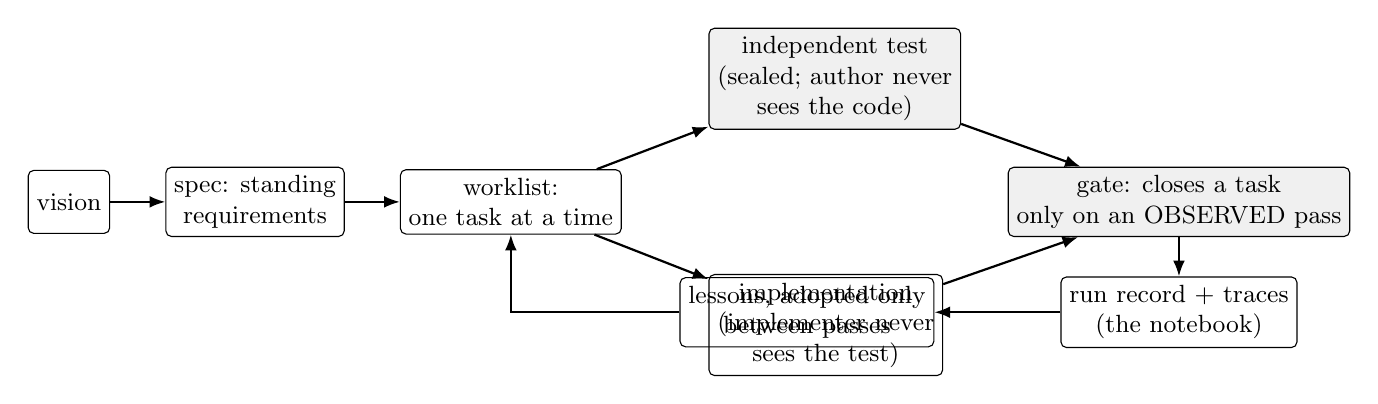
\begin{tikzpicture}[
  node distance=5mm and 7mm,
  box/.style={draw, rounded corners=2pt, align=center, font=\small, minimum height=8mm, inner sep=3pt},
  seal/.style={box, fill=black!6},
  arr/.style={-{Latex[length=2mm]}, thick}]
  \node[box] (vision) {vision};
  \node[box, right=of vision] (spec) {spec: standing\\requirements};
  \node[box, right=of spec] (worklist) {worklist:\\one task at a time};
  \node[seal, above right=of worklist, xshift=4mm] (test) {independent test\\(sealed; author never\\sees the code)};
  \node[box, below right=of worklist, xshift=4mm] (impl) {implementation\\(implementer never\\sees the test)};
  \node[seal, right=of worklist, xshift=42mm] (gate) {gate: closes a task\\only on an OBSERVED pass};
  \node[box, below=of gate] (record) {run record + traces\\(the notebook)};
  \node[box, left=of record, xshift=-9mm] (lessons) {lessons, adopted only\\between passes};
  \draw[arr] (vision) -- (spec);
  \draw[arr] (spec) -- (worklist);
  \draw[arr] (worklist) -- (test);
  \draw[arr] (worklist) -- (impl);
  \draw[arr] (test) -- (gate);
  \draw[arr] (impl) -- (gate);
  \draw[arr] (gate) -- (record);
  \draw[arr] (record) -- (lessons);
  \draw[arr] (lessons) -| (worklist);
\end{tikzpicture}
}
\end{center}

\begin{table}[h]
\centering
\small
\begin{tabular}{@{}p{4.2cm}p{9.6cm}@{}}  % claims: ignore-line
\toprule
Lab method & The loop \\
\midrule
Pre-registration & The specification: standing requirements, frozen at one approval before any code is written. Scope cannot drift mid-pass. \\
Blinded assessment & The independent test for each task, written by an author who never sees the implementation. The implementer never sees the test. \\
The lab notebook & The pass record and the traces: what was attempted, what closed, what was set aside, under which configuration. \\
A protocol amendment & A lesson: a captured observation that may change how the next pass runs, and is adopted only between passes, never during one. \\
The reviewer who signs off & The gate: a worklist tool with no model inside it, which closes a task only when it has itself observed the independent test pass. \\
\bottomrule
\end{tabular}
\caption{The mapping this paper teaches by. The right-hand column uses the plain words the text uses throughout; the project's own glossary maps each to its internal term.}
\label{tab:mapping}
\end{table}

\paragraph{Who can close a task.} Nothing that writes code can record that it passed. The worklist tool is the only writer of a task's state; it runs the independent test itself and reads the test runner's own report, never the runner's exit code, because exit codes conflate ``the test failed'' with ``the test never ran''. A gate that could not execute halts and says so; it is never retried as if the code were merely wrong, because that path burns the attempt budget on nothing and then sets a task aside with evidence of nothing. This distinction --- \emph{ran and failed} versus \emph{could not run} --- recurs in Section~\ref{sec:audit} as the shape of most of the defects we found.

\paragraph{The seal.} The independent test is sealed: a digest is recorded when it is authored, the gate refuses a test that changed after sealing, and the agent that implements is blocked by a hook from reading the sealed directory at all. When this paper needed the sealed suite re-run (Section~\ref{sec:biosim}), the run happened through the same referee tool the gate uses, over an archived copy of the pass-end commit, and the authors saw counts and test names only.

\paragraph{What the first pass looked like.} The first pass closed \claimunits{} tasks against a small spend-tracking library, in the order their requirements were declared, with each task's independent test passing on the tool's own observation (Figure~\ref{fig:timeline}). The timeline is \emph{reconstructed} from version control: each close is a commit whose subject names the task and the requirement it satisfies. Section~\ref{sec:limits} explains why the tool's own record of that pass carries a weaker label.

\begin{figure}[h]
\centering
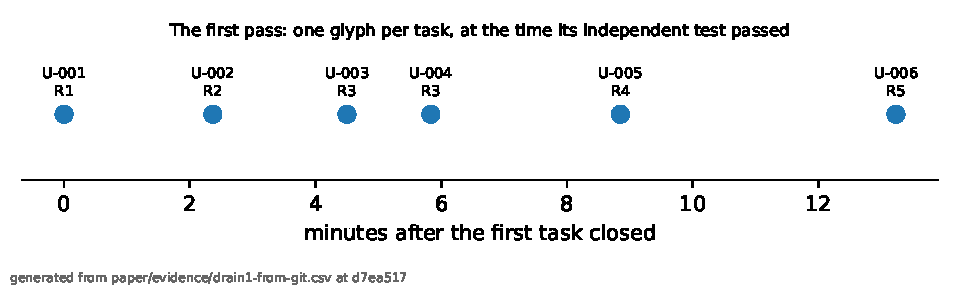
\includegraphics[width=\linewidth]{figures/timeline.pdf}
\caption{The first pass, reconstructed from version control: one glyph per task at the time its independent test passed. \claimunits{} tasks. Whether any task was set aside is not something version control records; the recovered record says none was (Section~\ref{sec:limits}).}
\label{fig:timeline}
\end{figure}

\section{The tool}\label{sec:tool}

The loop ships as a plugin for an agentic coding harness, with three command-line tools that contain no language model:

\begin{itemize}
\item \textbf{the worklist} (\texttt{register}) owns every task transition --- claim, seal, close, set aside --- and is the only thing that may close a task. It records the pre-claim commit so a task set aside can be restored exactly, and writes the pass record at the end of a pass.
\item \textbf{the referee} (\texttt{referee}) runs a project's sealed suite through a configured command, reads results in a fixed dialect, counts what arrived against what the suite declared, and signs a receipt only for a suite that passed with nothing skipped and nothing unaccounted for.
\item \textbf{the meter} (\texttt{spend}) enforces a declared spending cap; it was the loop's own first product, built by the first pass.
\end{itemize}

At the version this paper cites, the plugin's own suites for these tools run \claimplugintests{} assertions with \claimpluginfail{} failing (\emph{measured}: re-run for this paper in a scratch checkout of the tagged commit, not copied from a changelog); the worklist tool alone carries \claimregtests{} of them. That version is \texttt{aiadlc}~\claimpluginver{} (commit \texttt{\claimplugincommit{}}); the plugin was renamed \texttt{airdlc} after it, so later releases are published under that name. Installation is a plugin-marketplace add followed by one configuration key naming the project's referee command; the plugin's repository documents the first, and the evidence README gives the key and the command this paper used.

The tool is deliberately small. Its safety does not come from the agents being trustworthy; it comes from the fact that no agent in the loop can close its own work, and from the referee reading a report rather than an exit code. Section~\ref{sec:audit} is a list of the ways that small tool was nevertheless wrong.

\section{The worked experiment}\label{sec:biosim}

\paragraph{The question.} Human preproinsulin folds through three disulfide bonds. Mutations that disrupt or create a cysteine in proinsulin, C96Y among them, cause permanent neonatal diabetes through misfolding~\cite{stoy2007insulin}, and the Akita mouse's Ins2 C96Y allele is the classic disulfide-disrupting case~\cite{wang1999akita}. So a protein language model that has learned anything about this protein should treat those six positions as load-bearing. This is a question with a known answer, which is exactly what one wants from a worked example: if the loop had corrupted the number, the number would be wrong, not merely different.

\paragraph{The environment.} We wrap an ESM-2 650M scorer~\cite{lin2023esm} as an aviary environment~\cite{narayanan2024aviary}: the agent sees two tools, one that scores a single-residue substitution and one that embeds a sequence, and nothing else. Scores are masked-marginal log-odds~\cite{meier2021zeroshot}; the evaluator is frozen and its identity recorded. The sequence is fetched from UniProt~\cite{uniprot2023} by accession and cached; the cache is file content, not trusted input, and every value read from it is validated before it can reach a path or a URL.

\paragraph{The input, verified.} Before any number was re-computed we fetched the record fresh from the database with the cache bypassed and compared it, by digest, to the sequence the original run used: \claimseqlen{} residues, identical digest (\emph{measured}, fresh fetch, dated in the evidence file). The input is UniProt accession \texttt{\claimaccession{}} at database release \texttt{\claimuprelease{}}, with sequence SHA-256
\begin{center}\small\texttt{\claimseqsha{}}.\end{center}
\noindent Within this paper these three values appear only here and in the evidence file, by an explicit ruling: a digest over an enumerable identifier is a lookup, not a redaction, and the association between this protein and its public record is already published by the repository, so restating it for reproducibility creates no new one.

\paragraph{Results, re-measured.} Over the hash-verified input we re-ran the full single-substitution scan --- \claimsubs{} substitutions --- with the model identity, weights digest, device, seed and library versions recorded beside the numbers. Every headline value matched the original run to the reported precision, and all per-position means matched exactly. Within the mature protein (\claimmatsubs{} substitutions after the signal peptide), the six disulfide cysteines score \claimcysmean{} on average against \claimothermean{} for every other residue (Figure~\ref{fig:cysteines}); across the whole precursor, signal peptide included, the non-cysteine mean is \claimothermeanall{} instead, and the paper is careful throughout about which of the two a given number is. The re-run took \claimrerunsec{} seconds on an Apple GPU. The original run's own artifact reports \claimpubsec{} seconds (\emph{reported}). The model weights were \claimweightsgb{} bytes, digest recorded.

\begin{figure}[h]
\centering
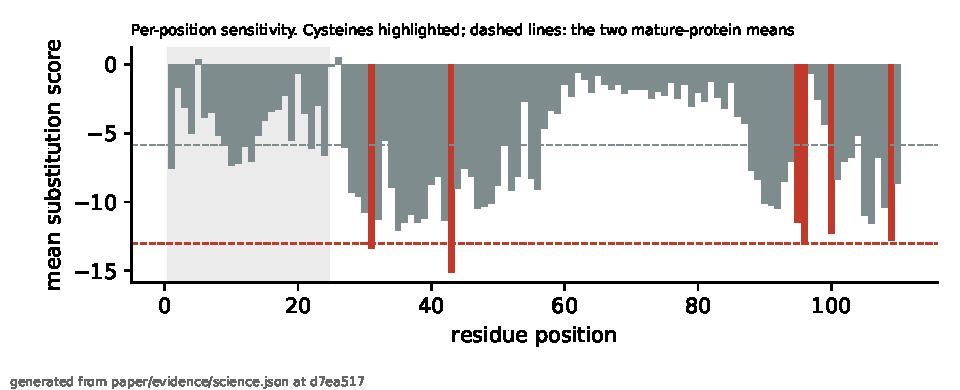
\includegraphics[width=\linewidth]{figures/cysteines.pdf}
\caption{Per-position mean substitution score across the \claimseqlen{}-residue sequence; cysteines highlighted; the signal peptide shaded. Dashed lines: the mature-protein means, \claimcysmean{} at the cysteines and \claimothermean{} elsewhere (\emph{measured}, re-run).}
\label{fig:cysteines}
\end{figure}

\paragraph{The agent's run.} A discovery agent given the environment and a one-paragraph objective chose \claimmeas{} measurements over \claimrounds{} rounds, at \claimpositions{} distinct positions, spending \claimtokens{} completion tokens in the rounds that recorded a count (\emph{reported}: counted from the run's own artifact, whose digest and size are in the evidence; \claimnotokens{} round recorded no token count and is reported as such, not as zero). Its round \claimcysround{} requested the six cysteines and two C-peptide positions together, so the cysteines were targeted from the start rather than arrived at: the objective named the protein, and where to look was prior knowledge the agent brought, not a finding it made. In its final write-up it listed \claimctrlnamed{} positions as tolerant controls, of which \claimctrlnamedcpep{} fall in the C-peptide --- cleaved out of mature insulin and poorly conserved --- as the scan's own region annotation defines it, the rest lying outside it. The agent never refers to that region; reading its choice as a C-peptide control is our interpretation of what it did, and the only thing \emph{reported} here is the list of positions. At the C-peptide positions among them, in sequence order, the re-run scan scores the alanine substitution at \claimctrlA{}, \claimctrlD{}, \claimctrlE{}, \claimctrlB{} and \claimctrlC{}, against \claimcysmean{} at the cysteines (\emph{measured}). Which positions to probe was the agent's choice, and is \emph{reported}; which substitution it tried at each is not in the evidence, so none is claimed. The run's trace exists in the project's trace store: \claimtraceroots{} root trace for the discovery run, one of the project's \claimtraceprojroots{} root traces, among \claimtracetotal{} traces in all (\emph{queried}, dated).

\paragraph{The independent tests, re-run.} The \claimunits{} tasks of the first pass carried \claimsealed{} independent tests. For this paper they were re-run through the referee over an archived copy of the pass-end commit, with every dependency declared: \claimsealed{} passed, \claimsealedfail{} failed, none skipped (\emph{measured}, re-run, dated). The referee also signed a receipt, and that signature is deliberately not part of the claim: it binds the tree the referee ran in, not the archived pass-end tree the suite was run over, so it attests the counts' provenance and not the code they were measured against. Its hash is recorded in the evidence file. The authors saw counts and test names only.

\section{What the audit found}\label{sec:audit}

We audited the loop's own trust core --- the worklist, the referee, the isolation guard around the science suite, and the seeder that feeds the demonstration dashboard --- across several review passes, and kept a table of every defect. They share one shape: \emph{a mechanism reports success while the property it exists to guarantee is absent.} Table~\ref{tab:taxonomy} (rendered in full as Figure~\ref{fig:taxonomy}) lists \claimtaxrows{} of them; every row cites the regression test that now pins it or says plainly that it has none (\emph{documented}: the check that builds this paper verifies each cited test exists). Those tests live in the repository's own suites, re-run for this paper: \claimscitests{} over the science environment, \claimwltests{} over the worklist tool, and \claimpapertests{} over the scripts that produce this paper's evidence (\emph{measured}, re-run, dated).

\begin{figure}[h]
\centering
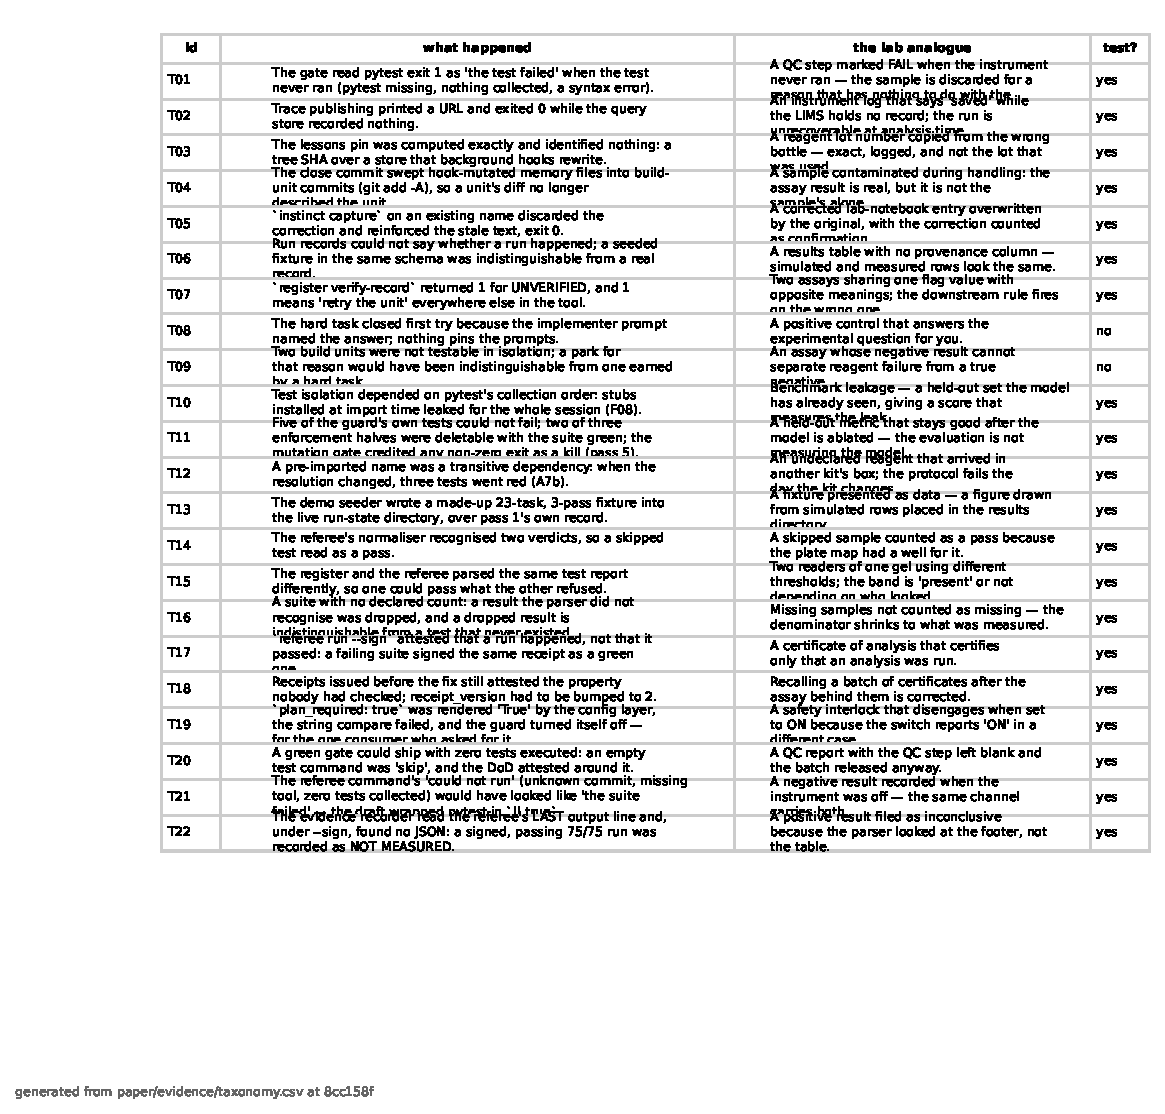
\includegraphics[width=\linewidth]{figures/taxonomy.pdf}
\caption{The failure-mode taxonomy: what happened, the laboratory analogue, and whether a test now pins it. Drawn from \texttt{taxonomy.csv}.}
\label{fig:taxonomy}
\end{figure}

\begin{table}[h]
\centering
\small
\begin{tabular}{@{}p{5.6cm}p{8.2cm}@{}}  % claims: ignore-line
\toprule
The shape & The laboratory analogue \\
\midrule
A gate read a runner's exit code, so ``could not run'' looked like ``ran and failed''. & A QC step marked FAIL when the instrument never switched on. \\
A test suite was green because a dependency happened to arrive through another package. & An undeclared reagent that came in another kit's box. \\
A guard's own tests could not fail; the mutation gate that checks the guard credited any non-zero exit as a kill. & A held-out metric that stays good after the model is ablated. \\
A demonstration seeder wrote a fixture into the live run directory, over the real record. & Simulated rows placed in the results directory. \\
A referee read a skipped test as a pass, and signed a receipt for a run that merely happened. & A certificate of analysis certifying only that an analysis was run. \\
A digest of an enumerable identifier was taken for a redaction. & Pseudonymisation that a lookup table reverses. \\
\bottomrule
\end{tabular}
\caption{Six of the \claimtaxrows{} shapes, chosen for their analogues. The full table is Figure~\ref{fig:taxonomy}.}
\label{tab:taxonomy}
\end{table}

Two of the rows are about building this paper. The referee command we wrote to re-run the sealed suite first wrapped the test runner in a construct that swallowed its exit status, so ``no tests collected'' would have printed nothing and read as a pass --- caught at the plan gate, before it ran. And the script that records the referee's verdict read the wrong output line under one flag, and recorded a signed, passing run as \emph{not measured}: a false negative in the safe direction, still false, and it would have hidden a real pass. We include them because a taxonomy of other people's mistakes is easy to write.

The mutation gate deserves a sentence, because it is how several of these were found~\cite{demillo1978mutation}. The isolation guard around the science suite is protected by a frozen catalogue of mutants --- small edits to the guard that a correct test suite must notice. A survivor means a property is no longer pinned by any test. Three review passes each found the same defect in different clothes (authentication of a module by a marker, then by its file path, then by its declared origin --- every attribute a fake can set), and each time the catalogue was extended rather than the count re-declared. The count is reported as live entries plus retired entries, never as a bare ratio, because a retargeted entry makes the count say something the catalogue cannot support: \claimmutkilled{} of \claimmutlive{} live mutants killed, with \claimmutretired{} retired against a stated reason.

\section{Limitations}\label{sec:limits}

\paragraph{Self-improvement is a mechanism, not a result.} The loop captures lessons between passes and pins the lesson set a pass ran under. This paper ran one pass. Pass-to-pass improvement was never measured, lessons have not been shown to change an outcome, and no sentence in this paper claims otherwise. Section~\ref{sec:next} says what measuring it would take.

\paragraph{The tool's own record of the first pass.} The demonstration seeder once wrote a made-up fixture --- more tasks, three passes, apparent improvement --- into the same live directory the loop writes to, in the main checkout, over the first pass's own record. The fixture depicted exactly the claim the previous paragraph forbids; the public dashboard page disclosed it; the seeder now refuses that directory (Section~\ref{sec:audit}). A copy of a record for the first pass was later recovered from a separate worktree. Its pre-claim chain checks out against history for all \claimchain{} tasks (each recorded pre-claim commit is exactly the parent of that task's close), it lists \claimclosed{} closed and \claimparked{} set aside, and its recorded register digest matches the register file beside it. None of that establishes \emph{when} it was written: a later reconstruction writing both files would also match, the tool's own provenance check predates the record's format and reports it unverified, and the tool is itself the artifact under study. We therefore label it \emph{recovered record; pre-claim chain verified; write-time provenance not established}, and the pass itself as \emph{reconstructed from version control}.

\paragraph{One evidence file is not pinned to the code that produced it.} A recorded commit only identifies the producing code if the working tree was that commit, and for one file we cannot show that it was. The plugin-suite counts were measured, on the date their label records, against a separate checkout of the tool's repository at the tag for version \claimpluginver{}, and that checkout no longer exists on the machine the rebuild ran on, so the file could not be regenerated with the rest. Its commit therefore predates later fixes to the producing scripts --- fixes that changed what some labels could mean --- and its values were not re-derived for this revision. Its counts keep the \emph{measured} label and the date they were re-run on, which is what that label asserts; what is missing is the stronger guarantee the other files now carry, that the commit named beside the numbers is demonstrably the code that produced them. Every other script-produced file in this paper was rebuilt, on a clean tree, by a producer that refuses to run on a dirty one.

\paragraph{Both the model and the agent already knew the answer.} The experiment was chosen because its answer is known, and that cuts the other way too: it establishes nothing about either system discovering anything. ESM-2's training set includes insulin, so the scan recovers a constraint the model has seen rather than predicting an unseen one. The agent was told which protein to study and requested the cysteines in its first round, before any measurement came back (Section~\ref{sec:biosim}), so its targeting is prior knowledge carried into the task, not an inference drawn from the scores. What the experiment tests is the loop: whether a known-correct number survives the machinery intact. A claim about discovery would need a protein held out of training and an objective that does not name the site of interest, and this paper makes none.

\paragraph{Compute and venue.} The science ran on an Apple GPU and a serverless inference endpoint. The venue that framed the work supplied no compute for it.

\paragraph{Budget enforcement never ran end to end.} The environment refuses to start a discovery run without a declared token price, and none has been supplied; the agent run reported above predates that enforcement.

\paragraph{Reproducibility of the original science numbers.} When the original numbers were computed, the sequence cache's read path had no integrity check. The re-run in Section~\ref{sec:biosim} used an input verified fresh against the database and matched the original on every value, which is why those values now carry a \emph{measured} label; the original artifacts alone would not have earned it.

\paragraph{A single pass, a small library.} \claimunits{} tasks against a spend tracker is a demonstration of the mechanism, not evidence about how the loop behaves on a large codebase or over many passes.

\section{Preconditions for measuring improvement}\label{sec:next}

No second pass was run for this paper, and nothing here executes one. Measuring improvement would need: a second pass on the same specification with the lesson set pinned by content (the current pin is a tree digest over a store that background hooks rewrite, so two passes with identical lessons can carry different pins); the two prompts --- the test author's and the implementer's --- pinned alongside the seed, because the first pass's hardest task closed first try, and its prompt named the answer (T08) --- which of those explains the other was never tested; a pre-declared outcome measure (tasks closed per attempt, or attempts to close) written down before the pass starts; and a run record whose authorship the tool's own provenance check can verify, which the tool now writes.

\appendix
\section{Claims table}
Every macro in this paper, its value, its label and the evidence field it resolves to. Generated by the claims check at build time.

% GENERATED by claims.py — do not edit
\begin{longtable}{@{}lp{2.6cm}p{3.2cm}p{5.6cm}@{}}
\toprule id & value & label & evidence (file:field) \\ \midrule \endhead
\texttt{subs} & 2,090 & measured (re\mbox{-}run, 2026\mbox{-}09\mbox{-}26) & \texttt{science.\allowbreak{}json:\allowbreak{}headline.\allowbreak{}substitutions} \\
\texttt{cysmean} & −13.02 & measured (re\mbox{-}run, 2026\mbox{-}09\mbox{-}26) & \texttt{science.\allowbreak{}json:\allowbreak{}headline.\allowbreak{}cysteine\_mean\_mature} \\
\texttt{othermean} & −5.85 & measured (re\mbox{-}run, 2026\mbox{-}09\mbox{-}26) & \texttt{science.\allowbreak{}json:\allowbreak{}headline.\allowbreak{}other\_mean\_mature} \\
\texttt{othermeanall} & −5.53 & measured (re\mbox{-}run, 2026\mbox{-}09\mbox{-}26) & \texttt{science.\allowbreak{}json:\allowbreak{}headline.\allowbreak{}other\_mean} \\
\texttt{matsubs} & 1,634 & measured (re\mbox{-}run, 2026\mbox{-}09\mbox{-}26) & \texttt{science.\allowbreak{}json:\allowbreak{}headline.\allowbreak{}n\_substitutions\_mature} \\
\texttt{seqlen} & 110 & measured (fresh fetch, 2026\mbox{-}09\mbox{-}26) & \texttt{science\mbox{-}input.\allowbreak{}json:\allowbreak{}published.\allowbreak{}length} \\
\texttt{ctrlA} & 1.53 & measured (re\mbox{-}run, 2026\mbox{-}09\mbox{-}26) & \texttt{science.\allowbreak{}json:\allowbreak{}headline.\allowbreak{}c\_peptide\_controls.\allowbreak{}62} \\
\texttt{ctrlB} & 1.08 & measured (re\mbox{-}run, 2026\mbox{-}09\mbox{-}26) & \texttt{science.\allowbreak{}json:\allowbreak{}headline.\allowbreak{}c\_peptide\_controls.\allowbreak{}79} \\
\texttt{ctrlC} & −0.10 & measured (re\mbox{-}run, 2026\mbox{-}09\mbox{-}26) & \texttt{science.\allowbreak{}json:\allowbreak{}headline.\allowbreak{}c\_peptide\_controls.\allowbreak{}83} \\
\texttt{ctrlD} & 0.18 & measured (re\mbox{-}run, 2026\mbox{-}09\mbox{-}26) & \texttt{science.\allowbreak{}json:\allowbreak{}headline.\allowbreak{}c\_peptide\_controls.\allowbreak{}70} \\
\texttt{ctrlE} & 0.17 & measured (re\mbox{-}run, 2026\mbox{-}09\mbox{-}26) & \texttt{science.\allowbreak{}json:\allowbreak{}headline.\allowbreak{}c\_peptide\_controls.\allowbreak{}72} \\
\texttt{rerunsec} & 9.60 & measured (re\mbox{-}run, 2026\mbox{-}09\mbox{-}26) & \texttt{science.\allowbreak{}json:\allowbreak{}runtime\_s} \\
\texttt{pubsec} & 7.30 & reported & \texttt{science.\allowbreak{}json:\allowbreak{}published\_runtime\_s} \\
\texttt{weightsgb} & 2,609,506,392 & measured (re\mbox{-}run, 2026\mbox{-}09\mbox{-}26) & \texttt{science.\allowbreak{}json:\allowbreak{}weights\_bytes} \\
\texttt{meas} & 66 & reported (artifact counted, 2026\mbox{-}09\mbox{-}26) & \texttt{agent\mbox{-}run.\allowbreak{}json:\allowbreak{}measurements} \\
\texttt{rounds} & 5 & reported (artifact counted, 2026\mbox{-}09\mbox{-}26) & \texttt{agent\mbox{-}run.\allowbreak{}json:\allowbreak{}rounds} \\
\texttt{tokens} & 15,115 & reported (artifact counted, 2026\mbox{-}09\mbox{-}26) & \texttt{agent\mbox{-}run.\allowbreak{}json:\allowbreak{}completion\_tokens\_total} \\
\texttt{notokens} & 1 & reported (artifact counted, 2026\mbox{-}09\mbox{-}26) & \texttt{agent\mbox{-}run.\allowbreak{}json:\allowbreak{}rounds\_without\_a\_token\_count} \\
\texttt{positions} & 34 & reported (artifact counted, 2026\mbox{-}09\mbox{-}26) & \texttt{agent\mbox{-}run.\allowbreak{}json:\allowbreak{}distinct\_positions} \\
\texttt{traceroots} & 1 & queried (2026\mbox{-}09\mbox{-}26) & \texttt{weave\mbox{-}count.\allowbreak{}json:\allowbreak{}run\_discovery\_root\_traces} \\
\texttt{tracetotal} & 36 & queried (2026\mbox{-}09\mbox{-}26) & \texttt{weave\mbox{-}count.\allowbreak{}json:\allowbreak{}project\_total} \\
\texttt{sealed} & 75 & measured (re\mbox{-}run, 2026\mbox{-}09\mbox{-}26) & \texttt{drain1\mbox{-}rerun.\allowbreak{}json:\allowbreak{}referee.\allowbreak{}total} \\
\texttt{sealedfail} & 0 & measured (re\mbox{-}run, 2026\mbox{-}09\mbox{-}26) & \texttt{drain1\mbox{-}rerun.\allowbreak{}json:\allowbreak{}referee.\allowbreak{}failed} \\
\texttt{units} & 6 & reconstructed & \texttt{drain1\mbox{-}from\mbox{-}git.\allowbreak{}csv:\allowbreak{}rows} \\
\texttt{chain} & 6 & recovered record; pre\mbox{-}claim chain verified & \texttt{drain1\mbox{-}record\mbox{-}check.\allowbreak{}json:\allowbreak{}pre\_claim\_matches} \\
\texttt{closed} & 6 & recovered record & \texttt{drain1\mbox{-}record\mbox{-}check.\allowbreak{}json:\allowbreak{}closed\_count} \\
\texttt{parked} & 0 & recovered record & \texttt{drain1\mbox{-}record\mbox{-}check.\allowbreak{}json:\allowbreak{}parked\_count} \\
\texttt{pluginver} & 0.64.0 & measured (re\mbox{-}run, 2026\mbox{-}09\mbox{-}26) & \texttt{plugin\mbox{-}tests.\allowbreak{}json:\allowbreak{}plugin\_version} \\
\texttt{plugincommit} & e54bb44 & measured (re\mbox{-}run, 2026\mbox{-}09\mbox{-}26) & \texttt{plugin\mbox{-}tests.\allowbreak{}json:\allowbreak{}commit} \\
\texttt{plugintests} & 219 & measured (re\mbox{-}run, 2026\mbox{-}09\mbox{-}26) & \texttt{plugin\mbox{-}tests.\allowbreak{}json:\allowbreak{}totals.\allowbreak{}run} \\
\texttt{pluginfail} & 0 & measured (re\mbox{-}run, 2026\mbox{-}09\mbox{-}26) & \texttt{plugin\mbox{-}tests.\allowbreak{}json:\allowbreak{}totals.\allowbreak{}failed} \\
\texttt{regtests} & 60 & measured (re\mbox{-}run, 2026\mbox{-}09\mbox{-}26) & \texttt{plugin\mbox{-}tests.\allowbreak{}json:\allowbreak{}suites.\allowbreak{}register.\allowbreak{}test.\allowbreak{}sh.\allowbreak{}run} \\
\texttt{taxrows} & 22 & documented & \texttt{taxonomy.\allowbreak{}csv:\allowbreak{}rows} \\
\texttt{scitests} & 328 & measured (re\mbox{-}run, 2026\mbox{-}10\mbox{-}08) & \texttt{repo\mbox{-}tests.\allowbreak{}json:\allowbreak{}suites.\allowbreak{}science/\allowbreak{}tests.\allowbreak{}passed} \\
\texttt{wltests} & 42 & measured (re\mbox{-}run, 2026\mbox{-}10\mbox{-}08) & \texttt{repo\mbox{-}tests.\allowbreak{}json:\allowbreak{}suites.\allowbreak{}.\allowbreak{}claude/\allowbreak{}skills/\allowbreak{}v2r\mbox{-}loop/\allowbreak{}scripts/\allowbreak{}tests.\allowbreak{}passed} \\
\texttt{papertests} & 122 & measured (re\mbox{-}run, 2026\mbox{-}10\mbox{-}08) & \texttt{repo\mbox{-}tests.\allowbreak{}json:\allowbreak{}suites.\allowbreak{}paper/\allowbreak{}tests.\allowbreak{}passed} \\
\texttt{mutlive} & 48 & measured (re\mbox{-}run, 2026\mbox{-}10\mbox{-}08) & \texttt{repo\mbox{-}tests.\allowbreak{}json:\allowbreak{}mutants.\allowbreak{}live} \\
\texttt{mutkilled} & 48 & measured (re\mbox{-}run, 2026\mbox{-}10\mbox{-}08) & \texttt{repo\mbox{-}tests.\allowbreak{}json:\allowbreak{}mutants.\allowbreak{}killed} \\
\texttt{mutretired} & 1 & measured (re\mbox{-}run, 2026\mbox{-}10\mbox{-}08) & \texttt{repo\mbox{-}tests.\allowbreak{}json:\allowbreak{}mutants.\allowbreak{}retired} \\
\bottomrule
\end{longtable}


\section{Reproduction}
Each producer refuses to run on a dirty working tree and records whether the tree was clean, so the commit an evidence file names is the code that wrote it rather than merely the commit that happened to be checked out. The science, input, agent-run, sealed-suite and first-pass files were all rebuilt from one such commit:
\begin{center}\small\texttt{\claimevcommit{}}\end{center}
\noindent The repository's own test and mutation counts are measured from the commit that carries this text, since a paper cannot be written before the tests it counts. The plugin-suite file is the exception and is discussed in Section~\ref{sec:limits}. At the commit above, the repository's evidence README lists, for each evidence file, the task that produced it and the exact command. Every script records its git commit, timestamp, inputs path, interpreter and library versions beside its output; the model re-run additionally records the model identity, cache revision and weights digest. The sealed suite is re-run with the referee command named in the README; the referee signs a receipt only for a suite that passed with nothing skipped and every declared result accounted for.

\bibliographystyle{plain}
\bibliography{refs}
\end{document}
